\documentclass{article}
\usepackage[francais]{babel}
\usepackage[UTF8]{inputenc}
\usepackage[T1]{fontenc}
\usepackage{graphicx}
\usepackage{fancyhdr}
\usepackage{eurosym}
\usepackage{color}
\usepackage{soul}

\pagestyle{fancyplain} \chead{}\lhead{\textit{Les Professionnels}} \rhead{\emph{\textit{Evasion}}}

\definecolor{pseudorouge}{RGB}{200, 50, 50}
\definecolor{pseudoblue}{RGB}{20,10,230}

\begin{document}
\thispagestyle{empty}
\begin{center}
\fontsize{21}{21}{\textbf{Rapport de Soutenance 2 \vspace*{0.2cm}\newline\textit{Evasion}}}
\end{center}

\vspace*{0.7cm}

\begin{center}
\fontsize{21}{21}{\textbf{- Les Professionnels/}}
\fontsize{21}{21}{\textbf{2013-2014 -}}
\end{center}

\vspace*{0.5cm}

\begin{center}

\includegraphics[scale=01.0]{evasion}
\end{center}

\vspace*{0.5cm}

\fontsize{14}{14}
\begin{center}
{Lenny \textcolor{pseudorouge}{\textit{"Le Noob"}} Danino - danino\_l}
\end{center}
\begin{center}
Louis \textcolor{pseudoblue}{\textit{"El Parain"}} Kédémos - kedemo\_l
\end{center}
\begin{center}
Anatole \textcolor{pseudoblue}{\textit{"Totonut"}} Moreau - moreau\_a
\end{center}
\begin{center}
Khalis Chalabi - chalab\_k
\end{center}

\begin{center}

\includegraphics[scale=00.20]{infini}
\end{center}

\newpage
\thispagestyle{empty}
\tableofcontents

\newpage
\fontsize{12}{12}
\pagenumbering{arabic}
\section{Introduction}

\newpage

\section{Avancements}
\subsection{Louis\textcolor{pseudoblue}{\textit{"El Parrain"}} Kedemos}

\subsubsection{Expérience personnelle}
\newpage

\subsection{Khalis Chalabi}

\subsubsection{Avancement du projet}

\newpage

\subsection{Lenny \textcolor{red}{"Le Noob"} Danino}
\subsubsection{Personnages/Décors}

\par
Les textures des personnages sont des éléments très important dans le jeu car elles sont ce qui est immédiatement regardé par les joueurs. Il faut qu’elles soient jolies et agréables sinon les joueurs ne voudront pas jouer au jeu. Ainsi nous avons décidé qu’il serait préférable de dessiner par-dessus des textures provenant d’images sur internet. Cela apporte un degré de réalisme non négligeable.
\newline
\newline
\underline{Réalisations:}

\par
\underline{Les textures et le code:}
\newline

\par
Premièrement il a fallu réaliser un modèle de base pour les personnages découpé avec Blender.  Ce logiciel est extrêmement utile mais je n’y avais jamais touché et il m’a donc fallu l’aide de Louis et de tutos pour parvenir à me débrouiller suffisamment. Nous avons préféré rendre notre personnage cubique. C’était intéressant à faire car cela nécessitait de visualiser l’ensemble dans l’espace comme lorsqu’on découpe un cube.
\begin{center}
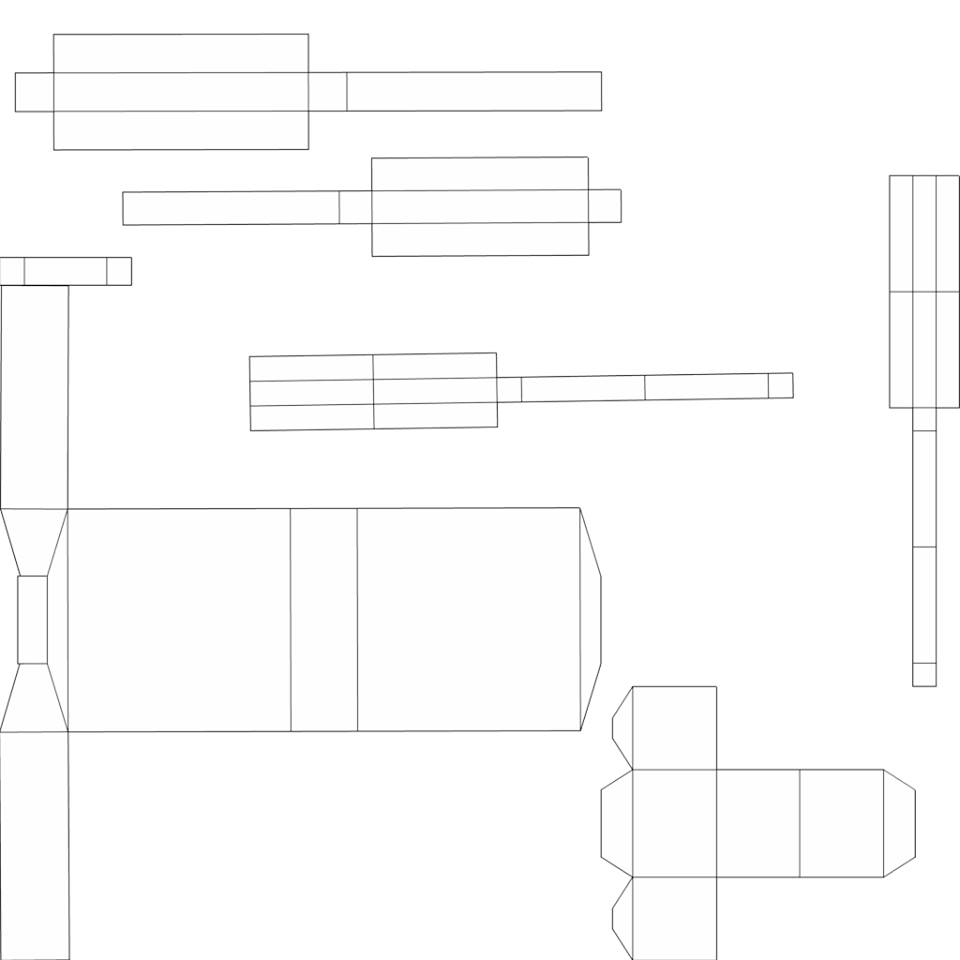
\includegraphics[scale=0.3]{decoupe.jpg}
\end{center}
\newpage
En me basant sur le modèle j’ai pu créer les textures de 2 personnages. J’ai utilisé Photoshop, qui comme Blender m’était entièrement inconnu, pour la correction des images et la découpe. Puis j’ai visualisé le résultat avec Blender. Je vous présente donc le Pnj des prisonniers :
\newline

\begin{center}
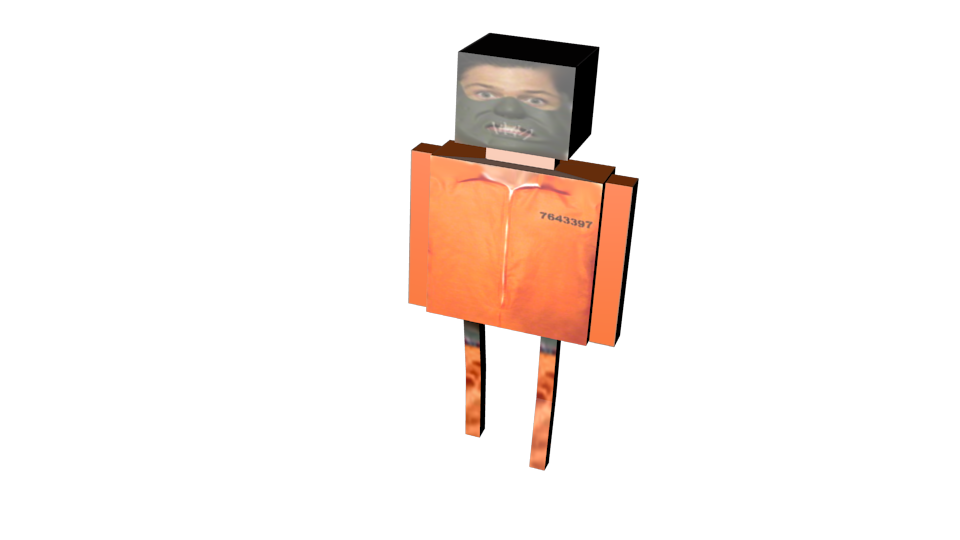
\includegraphics[scale=0.8]{prisonnierblend.png}
\end{center}
\begin{center}
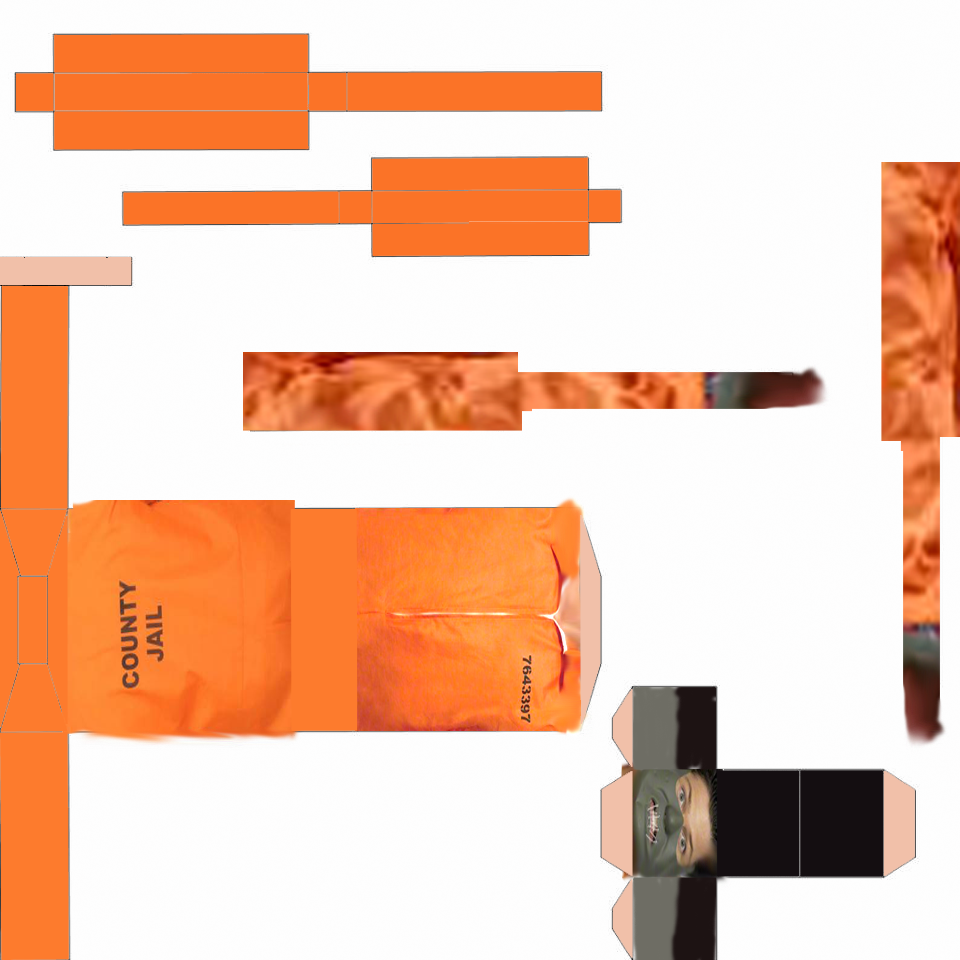
\includegraphics[scale=0.2]{prisonnier.png}
\end{center}
\newpage
Et voici un des ennemis en dehors de la prison : 
\begin{center}
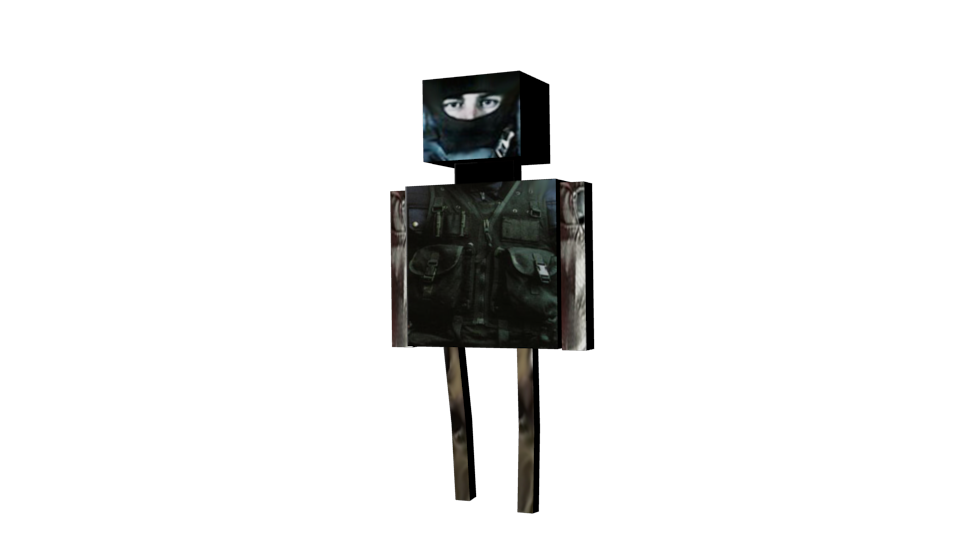
\includegraphics[scale=0.8]{ennemidehorsblend.png}
\end{center}
\begin{center}
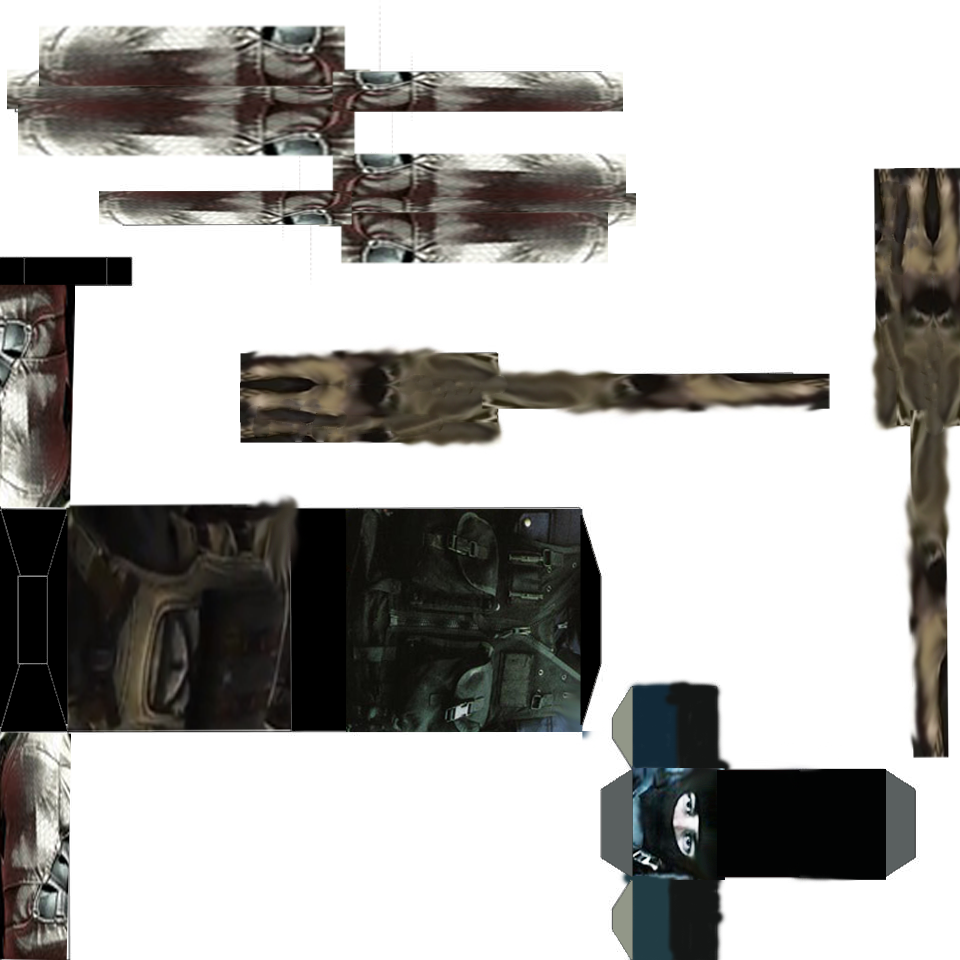
\includegraphics[scale=0.2]{ennemidehors.png}
\end{center}
\par
Cependant dessiner des personnages reste un aspect graphique. J’ai dû en effet toucher au code des classes pour pouvoir les insérer. Avec l’aide de Khalis, qui s’est occupé d’autres personnages, j’ai donc terminé les classes Pnj, Objets Utilitaires et Outils.
De même je m’étais occupe dans la première soutenance des classes Décors, Murs et Objets. Pour parfaitement les terminer j’ai dû effectuer les mêmes étapes que pour les personnages.
\newpage
Voici le modèle des murs :
\begin{center}
\includegraphics[scale=0.5]{mur_patron.png}
\end{center}
Voici une des textures utilises :
\begin{center}
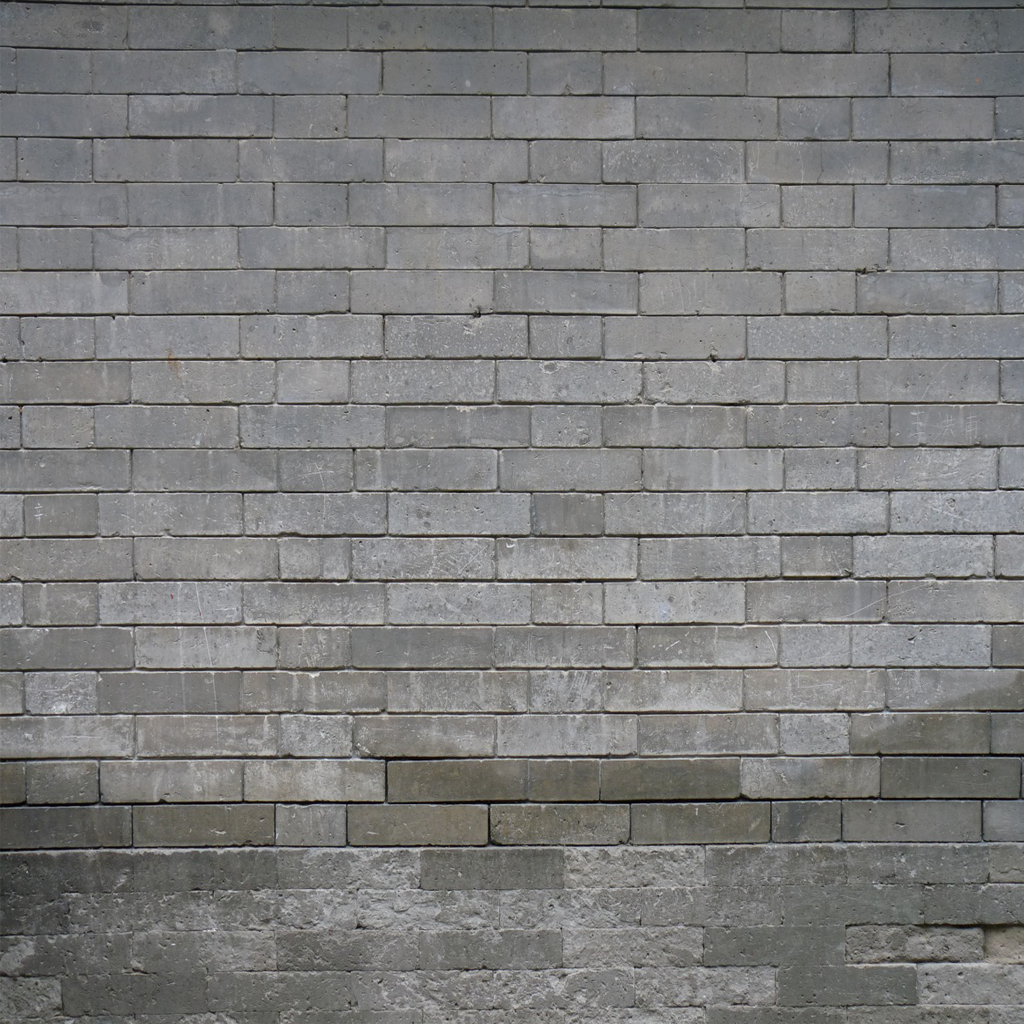
\includegraphics[scale=0.5]{mur_brique.png}
\end{center}
\subsubsection{Et après ?}
\par
Pour notre troisième soutenance je vais me fixer quelques objectifs à atteindre :
\newline

\par
\underline{Le multijoueur}
\newline
\par
Je compte terminer le multijoueur car même si aujourd'hui il est fonctionnel, je compte l'améliorer. Cela me permettra de progresser dans le code aussi.
\newline

\par
\underline{Les sons}
\newline
\par
Je compte rajouter des sons pour que l'ambiance du jeu soit complète lors de la troisième soutenance avec l’aide d’Anatole.
\newline

\par
\underline{L'éditeur de map}
\newline
\par
Enfin, je compte participer à l'édition des maps pour donner une dimension à notre jeu.
\newline

\par
\underline{Remerciements}
\newline
\par
Comment ne pas terminer encore une fois sur des remerciements à mon groupe qui reste soudé malgré nos différents? C'est donc pour cela que je remercie notre leader Louis qui soude quotidiennement notre équipe et nous encourage lorsque certains problèmes sont rencontrés, notre visionnaire Anatole qui aide à la projection du projet ainsi qu'à son aboutissement et toujours Khalis qui amène la bonne humeur tous les jours.

\newpage

\subsection {Anatole\textcolor {pseudoblue} {\textit {"Totonut"}} Moreau}
\newpage
\begin{tabular}{|c|p{2cm}|p{2cm}|p{2cm}|}


\hline
& Première soutenance & Deuxième soutenance & Troisième soutenance\\ 
\hline

Codage décors & 70\% & 100\% & 100\%\\
\hline
Codage objets & 70\% & 100\% & 100\%\\
\hline
Codage personnages & 70\% & 90\% & 100\%\\
\hline

Graphismes 2D/3D & - & 60\% & 100\%\\
\hline

Site web & 70\% & 100\% & 100\%\\
\hline

Son & 20\% & 80\% & 100\%\\
\hline

Collisions & - & 50\% & 100\%\\
\hline

Affichage & 70\% & 100\% & 100\%\\
\hline

Boucle de jeu & - & 50\% & 100\%\\
\hline

Interaction entre éléments du jeu & 20\% & 70\% & 100\%\\
\hline

Menu & 50\% & 100\% & 100\%\\
\hline

Réseau & - & 100\% & 100\%\\
\hline

Multijoueur & - & 60\% & 100\%\\
\hline

\end{tabular}

\section{Conclusion}

\end{document}
